\section{Controller}
\label{sec:controller}

The controller is a centralized web server exposing the HTTP REST interfaces  described in \Cref{tab:controller-rest} to interact with the public audience, the attacker and the bot.
In particular, the public audience is provided with the \textit{fake landig page} in \Cref{fig:controller-fake-landingpage}, the attacker with the  \textit{botnet management dashboard} in \Cref{fig:controller-botnet-dashboard} and the bot with a subset of \textit{HTTP REST APIs}.

\begin{table}%
\caption{Controller HTTP REST API}
\label{tab:controller-rest}
\begin{minipage}{\columnwidth}
\begin{center}
\begin{tabular}{clcl}
  \toprule
  METHOD & RESOURCE & CONTENT & DESCRIPTION \\
  GET    & /        & HTML    & Shows the fake landing page. \\
  GET    & /admin   & HTML    & Shows the botnet management dashboard. \\
  GET    & /init    & JSON    & Returns the controller configuration.   \\
  GET    & /command & JSON    & Returns the next command to execute. \\
  POST   & /report  & JSON    & Saves the bot report. \\
  \bottomrule
\end{tabular}
\end{center}
\end{minipage}
\end{table}

The content of the landing page must be such as to arouse in visitors both trust and indifference. In this way the visitor does not alarm and pass through without having any interest to further explore the website.

\begin{figure}[tp]
  \centering
  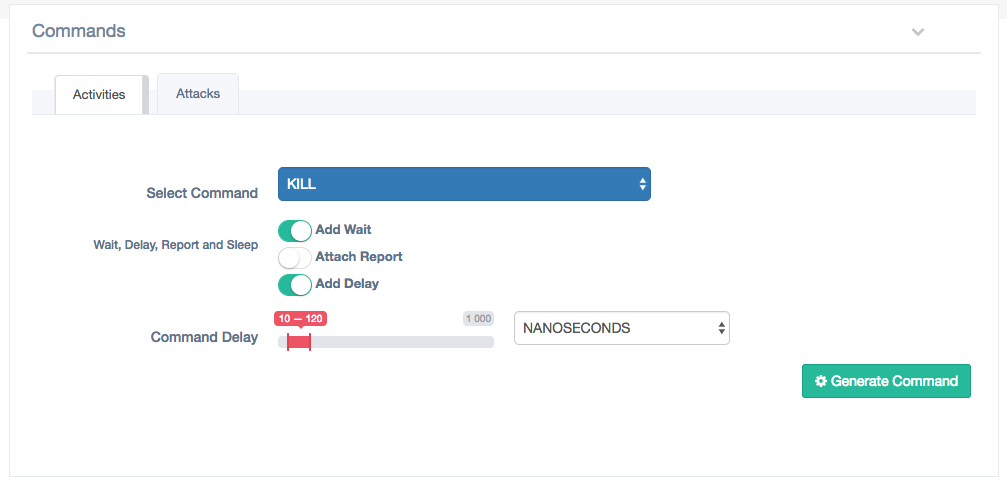
\includegraphics[scale=0.2]{./fig/commandsWUI.png}
  \caption{The fake landing page at \texttt{/index.html}.}
    \label{fig:controller-fake-landingpage}
\end{figure}

The botnet management dashboard provides the attacker with convenient forms to generate bot local configuration, submit controller-specific configuration and commands. 
Furthermore, all saved bot reports are stored in \texttt{/controller/data/report} as \texttt{report.\$\{botIP\}.json}.

\begin{figure}[tp]
  \centering
  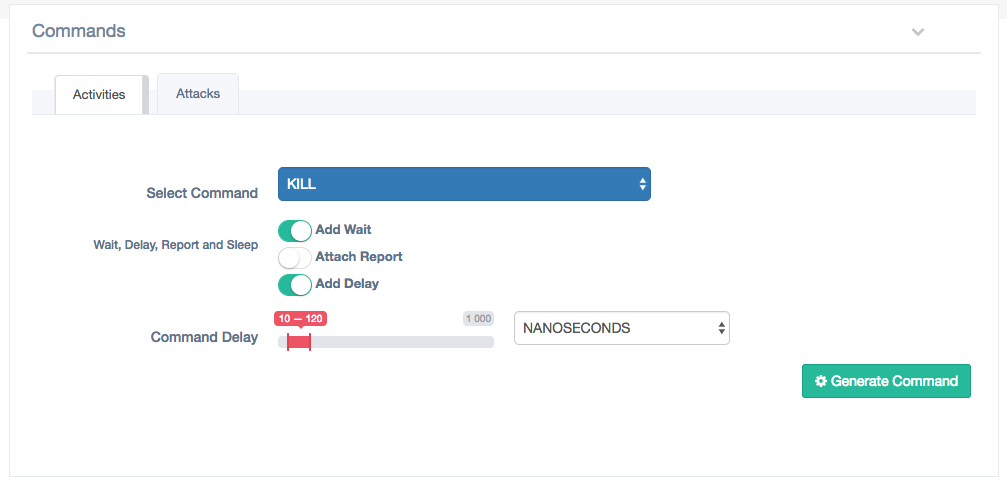
\includegraphics[scale=0.2]{./fig/commandsWUI.png}
  \caption{The botnet management dashboard at \texttt{/admin.html}.}
    \label{fig:controller-botnet-dashboard}
\end{figure}


